\documentclass[10pt,a4paper]{article}

\usepackage[ngerman]{babel}
\usepackage[colorinlistoftodos]{todonotes}
\usepackage[backend=biber,style=numeric]{biblatex}
\usepackage{graphicx}
\usepackage{float}

\addbibresource{bib.bib}

\title{Schallortung}
\author{Robin Heinemann\\ Jaro Habiger}
\date{\today}

\begin{document}
  \maketitle
  \begin{abstract}
  \todo{Wahrscheinlich Jaro: write abstract}
  \end{abstract}
  \thispagestyle{empty}
  
  \newpage
  \tableofcontents
  \thispagestyle{empty}
  
  \newpage
  \setcounter{page}{1}
  %begin the content
  
  \section{Problematik}
	\todo{Jaro: teilweise neuer text}
    Der Mensch hat die Fähigkeit, direktional zu hören, also die RIchtung zu bestimmen aus der ein Geräusch kommt. Dies bringt ihm enorme Vorteile bei der Erkennung von gesprochener Sprache und bei anderen akustischen Aufgaben. Diese Fähigkeit auf eine technische Apparatur zu übertragen und die Vorteile des räumlichen Hörens auch für diese nutzbar zu machen, hätte viele Anwendungsgebiete, die unser alltägliches Leben erleichtern könnten.\\
  Ein gutes Beispiel für eine Solche Anwendung wäre ein Rettungsroboter, der Hilfesuchende Menschen anhand von Hilferufen lokalisiert. 
  Jedoch sind auch Anwendungen aus komplett anderen Anwendungsbereichen 
  \section{Bestehende Lösungen} \todo{Check}
  Es gibt verschiedene Ansätze, die die verschiedenen Aspekte des direktionalen Hörens auf eine technische Apparatur übertragen. Diesen begegnen wir in unserem alltäglichen Leben relativ häufig. Die einfachste Form eines solchen Verfahrens ist das Richtmikrofon. Dieses führt allerdings keine aktive Ortung durch sondern kann lediglich in eine bestimmte Richtung besonders gut Schall aufnehmen. Um diese Fähigkeit in eine Richtungsbestimmung umzuwandeln müsste man also das Richtmikrofon drehen, oder es auf eine andere Weise aktiv nach der Schallquelle ausrichten. Ein weiterer Ansatz, dem wir in unserem alltäglichen Leben sehr viel häufiger begegnen, steckt in fast allen Mobiltelefonen. Diese filtern beim Telefonieren verschiedene Umgebungsgeräusche aus dem Mikrofonsignal, um die Sprachqualität zu verbessern. Die hierzu verwendeten Verfahren sind allerdings meist eher einfach gehalten, und erlauben keine wirkliche Bestimmung der Herkunftsrichtung eines Geräusches. Man kann sich dieses Verfahren sehr gut als ein Richtmikrofon vorstellen, das einen gewissen Bereich hat, in dem es sehr empfindlich ist, wohingegen es in anderen Bereichen sehr unempfindlich ist. Bei dieser Technik passiert ein Teil des Verfahrens in der Signalverarbeitung, also nach der eigentlichen Schallwandlung durch das Mikrofon. Hierdurch unterscheidet sich dieser Ansatz deutlich von dem des Richtmikrofones. Allerdings können auch mithilfe dieser Störgeräuschunterdrückung noch keine Positionen ermittelt werden. Auch moderne Hörgeräte verwenden ein ähnliches Verfahren, welches allerdings auch bei einer weiteren Distanz zwischen Mikrofon und Schallquelle funktioniert, und der gesuchten Lösung somit näher kommt. Sowohl die Geräuschunterdrückung in Handys, als auch die Filtertechniken in Hörgeräten verwenden meist zwei oder drei Mikrophone.
  \begin{figure}
  	\centering
  	\includegraphics[width=0.35\linewidth]{akusticCamera}
  	\caption{Ein Beispiel für eine akustische Kamera \cite{camera}}
  	\label{fig:camera}
  \end{figure}
  Eine andere existierende Lösung ist die akustische Kamera (siehe Abb. \ref{fig:camera}). Sie wird dazu verwendet, lärm-emittierende Positionen an Produkten zu finden, um diese optimieren zu können \cite{camera}. Die akustische Kamera verwendet allerdings bedeutend mehr Mikrofone als die anderen Verfahren. Einige Modelle verwenden mehr als 350 Mikrofone \cite{nmics}. Da uns alle vorhandenen Lösungen nicht zufrieden gestellt haben wollten wir ein eigenes Verfahren nur akustischen Richtungsbestimmung entwickeln, dass schon mit einer geringen Anzahl von Mikrofonen eine komplette Richtungsbestimmung ermöglicht.
  \section{Konzept} \todo{Jaro: Menschliches Gehöhr einbringen}
  \todo{was über die Analogie zum Menschen Schreiben}
      \subsection{Modul 1: Eingabe/Aufnahme}
      \subsection{Modul 2: Signal aufteilen}
      \subsection{Modul 3: Ortung}
      \subsection{Modul 4: Ausgabe}
  \section{Umsetzung der einzelnen Module} \todo{Jaro: Bleibt, Ortung -> Richtung}
      \subsection{Simulation (Modul 1)}
      \subsection{Hardware (Modul 1)}
      \subsubsection{Mikrofone}
      \subsubsection{Audio Interface}
      \subsubsection{Software}
      \subsection{Fourier-Transformation (Modul 2)}
      \subsection{Ortungsmodul (Modul 3)}
      \subsection{Ausgabemodul (Modul 4)}
      \subsection{Testen der einzelnen Module}
  \section{Eindimensionale Richtungsbestimmung} \todo{Robin: Bleibt, Ortung -> Richtung}
  Um den Algorithmus, der aus den Phasendifferenzen den Ort zurückrechnet zu entwickeln haben wir mit der
einfachsten Stufe der Ortung, die eindimensionale Ortung, angefangen:
	\begin{figure}
		\centering
        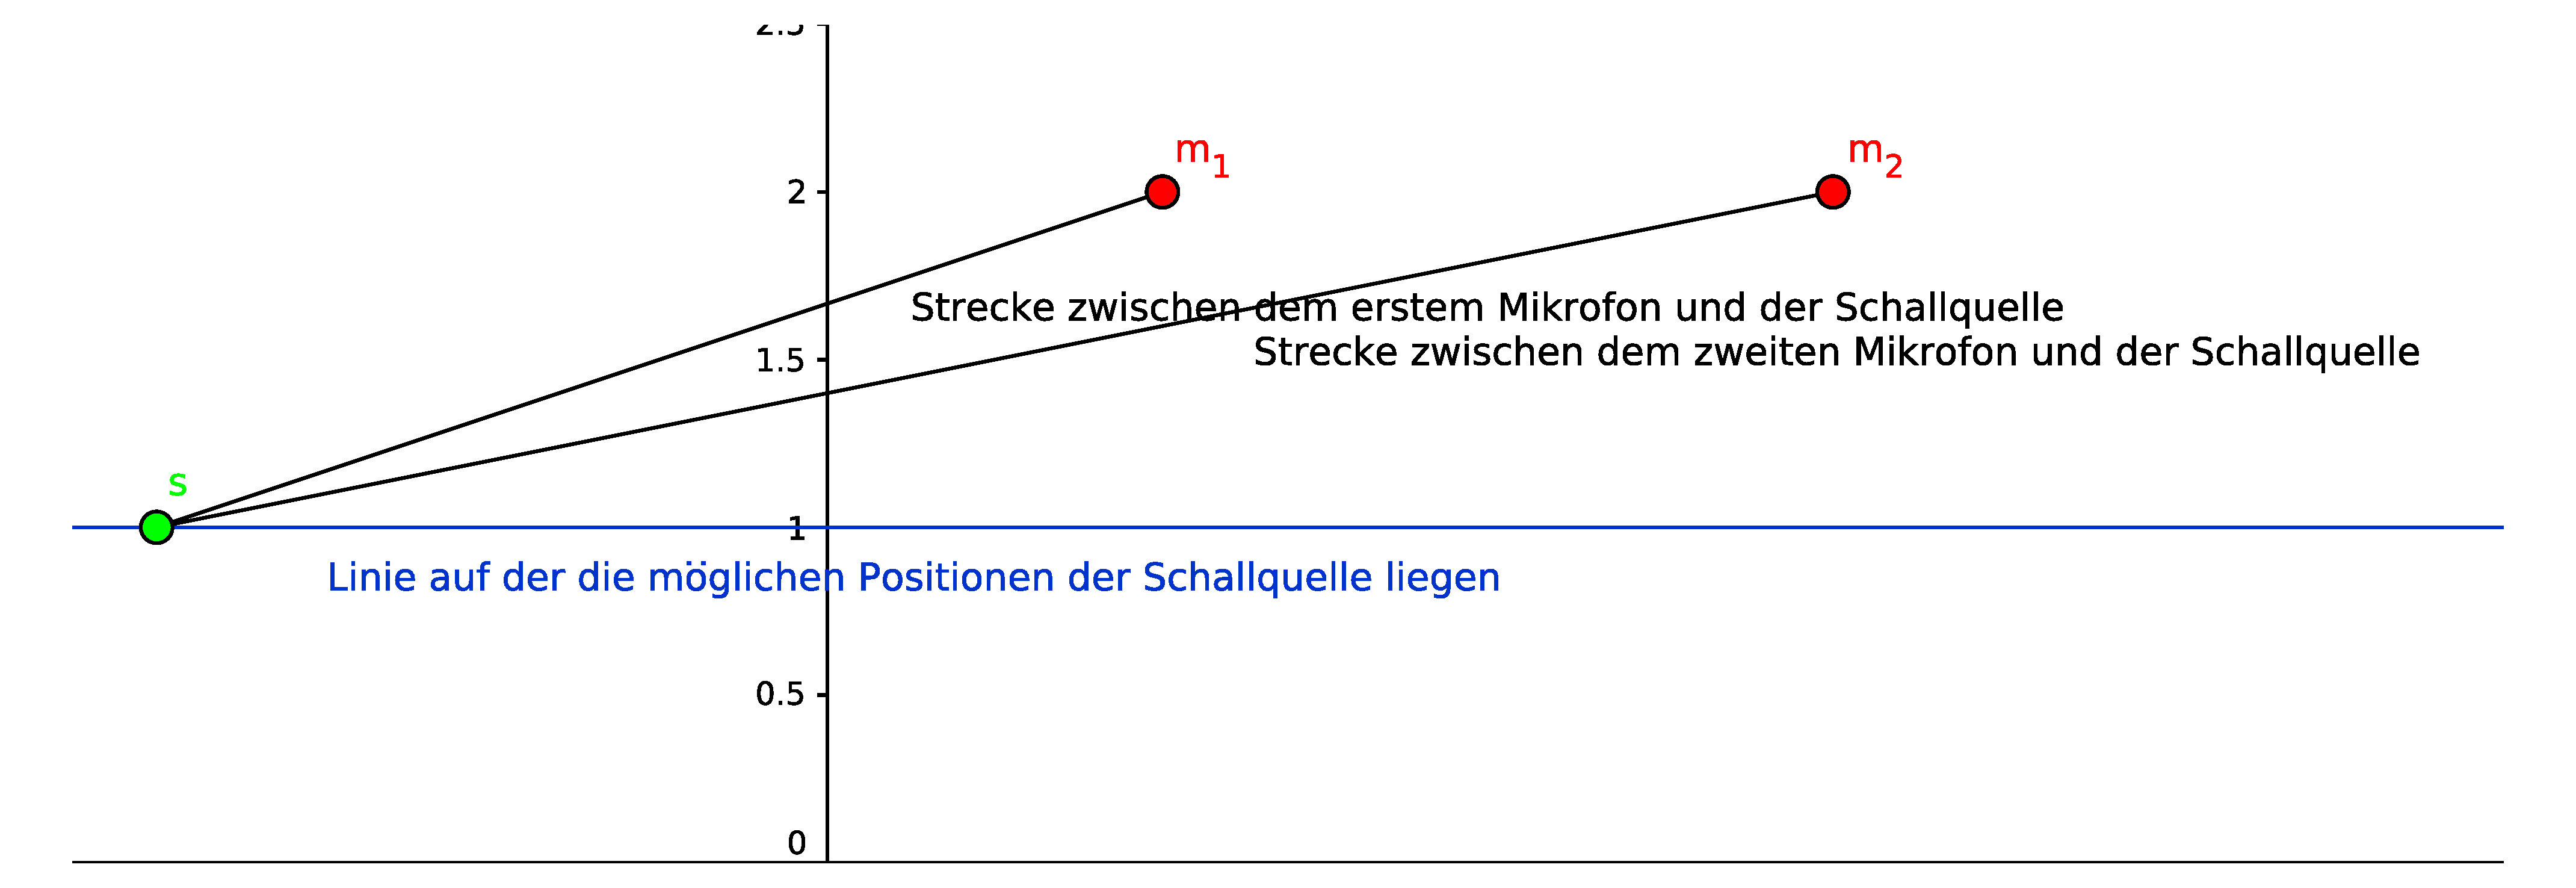
\includegraphics[width=\linewidth]{skizze1d}
        \caption{Skizze einer eindimensionalen Ortung}
	\end{figure}
  \section{Zweidimensionale Ortung} \todo{Robin: Bleibt, Ortung -> Richtung, analytisch -> numerisch}
      \subsection{Erweiterung der Theorie}
      \subsection{Analytisches Lösen des gleichungssystems}
  \section{Dreidimensionale Ortung} \todo{Robin: Neu, numerische mit least squares}
      \subsection{erweiterterung der Theorie}
      \subsection{Numerisches Lösen des Gleichugssystems}
  \section{Evaluation} \todo{Beide: Neu, echte Messungen einbauen}
      \subsection{Simulation}
      \subsection{Praxis}
  \section{Ausblick} \todo{Beide: Neu, 8mics ja, 38 verschweigen}
  \section{Fazit} \todo{Beide: neu, Richtung geht voll gut}
  
  \pagebreak % Quellen und co
  \pagenumbering{roman}
  \setcounter{page}{1}
  \printbibliography
\end{document}